\section{Архитектура моделей}\label{sec:model_architecture}

В этом разделе заданы параметрические блоки малой рекурсивной схемы (tiny recursive model, TRM) в
связке с обучением по меткам оракульного времени остановки, а также модификация, в которой к
рекурсии подключается предобученная малая языковая модель (small language model, sLLM). Смысл
объектов \(\tau^\star\) и последовательностей \(\{Z_{t,k}\}\), \(\{Q_{t,k}\}\), \(\{\widehat
p_{t,k}\}\) согласуется с разд.~\ref{sec:recursive_process}; здесь они конкретизируются указанием
наборов обучаемых параметров.

\subsection{Tiny Recursive Model с разметкой оракула}\label{ssec:arch_trm_oracle}

\textbf{Оператор рекурсивного ядра.} Для каждого внутреннего шага задаётся отображение
\begin{equation}
  \mathcal U_{\theta}:\ \R^{d_z}\times\R^{d_c}\times\Delta^{V-1}\rightarrow\R^{d_z},
  \qquad
  Z_{t,k+1}=Z_{t,k}+\mathcal U_{\theta}(Z_{t,k},C_t,Q_{t,k}), \quad k=0,\ldots,K-1,
  \label{eq:trm_residual_kernel}
\end{equation}
что задаёт параметрическую версию блока~\eqref{eq:recursive_update} в виде остаточного обновления;
\(C_t\in\R^{d_c}\) может быть функцией префикса и не изменяться внутри цикла.

\textbf{Чистая TRM-ветка без внешней sLLM.} Префикс кодируется одним параметрическим кодировщиком
(эмбеддинги токенов и возможные свёрточные/транзиентные блоки малой глубины):
\begin{equation}
  Z_{t,0}=E_{\phi^{(\mathrm{trm})}}(X_{1},\ldots,X_t),\qquad 
  \phi^{(\mathrm{trm})}\in\Phi_{\mathrm{trm}} .
  \label{eq:trm_embed_prefix}
\end{equation}

\textbf{Прогностическая голова.} По текущей скрытой переменной строится вектор логитов и
распределение на словаре:
\begin{equation}
  Q_{t,k}=\operatorname{softmax}\bigl(f_{\eta}(\cdot,Z_{t,k},C_t)\bigr),
  \label{eq:lm_head_general}
\end{equation}
то есть параметрическая версия связи~\eqref{eq:softmax_distribution} с дополнительным контекстным
входом \(C_t\); семейство \(f_{\eta}(\cdot,Z_{t,k},C_t)\) задаёт одно и то же отображение
\(\R^{d_z+d_c}\rightarrow\R^V\) в зависимости от аргумента \(a\) (строчное матричное умножение
после конкатенации признаков).

\textbf{Голова времени останова.} Собирается вектор признаков \(\mathbf g_{t,k}=R_{\psi}(\mathbf
h_{t,k})\),
\(\mathbf h_{t,k}=\bigl(Z_{t,k},Q_{t,k},\text{diag}(Z_{t,k})\bigr)\) --- здесь \(\text{diag}(Z_{t,k})\)
обозначает вектор из компонент \(Z_{t,k}\) (покомпонентное дополнение к признакам); после выбора
фиксированного конкатенированного или иного агрегирования статистик (как множество \(\{S_{t,k}\}\)
в~\eqref{eq:information_flow}) и задаётся
\begin{equation}
  \widehat p_{t,k}(\cdot)=\operatorname{softmax}\bigl(W_{\omega}\mathbf g_{t,k}+b_{\omega}\bigr),
  \qquad (\omega)=(W_{\omega},b_{\omega},\psi),\ \omega\in\Omega.
  \label{eq:stop_head_param}
\end{equation}
Форма \(\Pi_{\omega}\), используемая в тексте экспериментов как «голова модели времени», совпадает
с параметрическим семейством на \(\{0,\ldots,K\}\) после фиксации размерности выходного слоя.

\textbf{Разметка оракула.} После вычисления всех \(\{Q_{t,j}\}_{j=0}^{K}\) и наблюдения
\(X_{t+1}\) по формулам~\eqref{eq:nll_loss}--\eqref{eq:oracle_stopping_time} получают число
\(\tau_t^\star\). Обучение головы~\eqref{eq:stop_head_param} задаётся, например, перекрестной
энтропией между \(\widehat p_{t,k}(\cdot|\omega)\) и индикатором точечной метки \(\tau_t^\star\)
(или сглаженной разметкой, см.~\ref{sec:dist_families} и~\eqref{eq:distribution_loss});
прогностическое ядро и LM-голова обучаются по потере~\eqref{eq:nll_loss} на выбранных шагах. На
этапе вывода оракульная разметка не используется: применяется
правило~\eqref{eq:real_stopping_rule} поверх \(\widehat p_{t,k}\).

\begin{figure}[H]
\centering
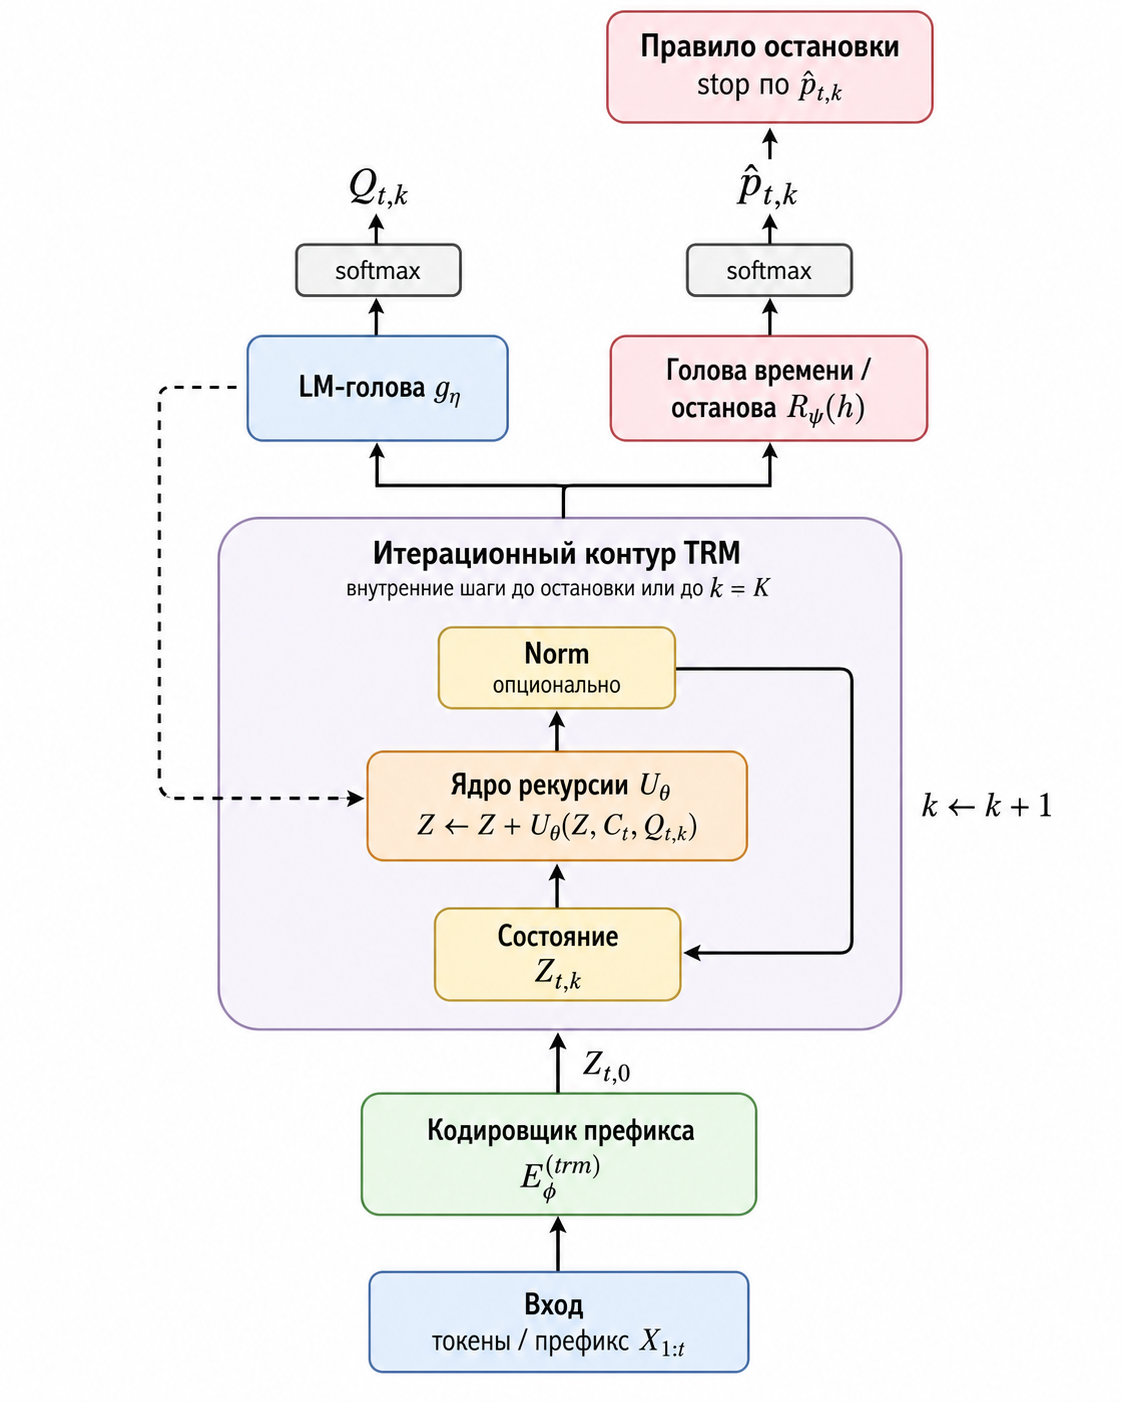
\includegraphics[width=\linewidth]{simple}
\caption{Структура сети чистого TRM (без внешней sLLM): кодировщик префикса, остаточное ядро
\(\mathcal U_{\theta}\) с итерациями по \(k\le K\), LM-голова и голова времени, минимальное
правило остановки по \(\widehat p_{t,k}\). Разметка оракула \(\tau_t^\star\) и совместное обучение
блоков описаны текстом выше; на схеме показан только вычислительный граф.}
\label{fig:arch_trm_oracle}
\end{figure}

Рисунок~\ref{fig:arch_trm_oracle} согласуется с
записью~\eqref{eq:trm_residual_kernel}\,--\,\eqref{eq:stop_head_param}: многократные шаги по
\(k\), использование распределения \(Q_{t,k}\) во входном наборе ядра \(\mathcal U_\theta\) и
построение голов после формирования скрытого состояния.

\subsection{sLLM перед рекурсивным ядром}\label{ssec:arch_sllm_trm}

В иной конфигурации префикс сначала пропускается через предобученную малую языковую модель,
фиксирующую промежуточное представление последнего токена (или среднее по последним \(m\) позициям):
\begin{align}
  h_t &= \mathrm{sLLM}_{\phi^{\mathrm{(s)}}}(X_{1},\ldots,X_t),\qquad 
  h_t\in\R^{d_h},\\
  Z_{t,0} &= P_{\psi}(h_t), \qquad P_{\psi}:\ \R^{d_h}\rightarrow\R^{d_z},\ \psi\in\Psi.
  \label{eq:sllm_to_trm}
\end{align}
Параметры \(\phi^{\mathrm{(s)}}\) чаще замораживают или ограниченно корректируют; главная
добавочная связь --- проектор \(P_\psi\).
Дальше задаются те
же~\eqref{eq:trm_residual_kernel},~\eqref{eq:lm_head_general},~\eqref{eq:stop_head_param}, при
необходимости с разделением параметров между «внешней» и чистой TRM-схемами.

\textbf{Необязательный LoRA.} В качестве дешёвой адаптации вместо или вместе с полным изменением
\(\phi^{\mathrm{(s)}}\) в промежуточных линейных слоях sLLM фиксируют низкоранговые приращения
коэффициентов в представлении \cite{hu2021}: матрицы в слоях заменяют на \(W{+}\alpha\,B^{\top}A\)
с малыми рангами \(A\in\R^{r\times d_{\mathrm{in}}}\), \(B\in\R^{r\times d_{\mathrm{out}}}\),
\(r\ll\min\{d_{\mathrm{in}},d_{\mathrm{out}}\}\). Эти дополнительные параметры относятся к
множеству \(\Phi_{\mathrm{adapt}}\subset\Phi_{\mathrm{trm}}\cup\Psi\); обозначение \emph{LoRA} в
работе сохраняется как принятое в литературе имя метода без русского перевода.

\begin{figure}[H]
\centering
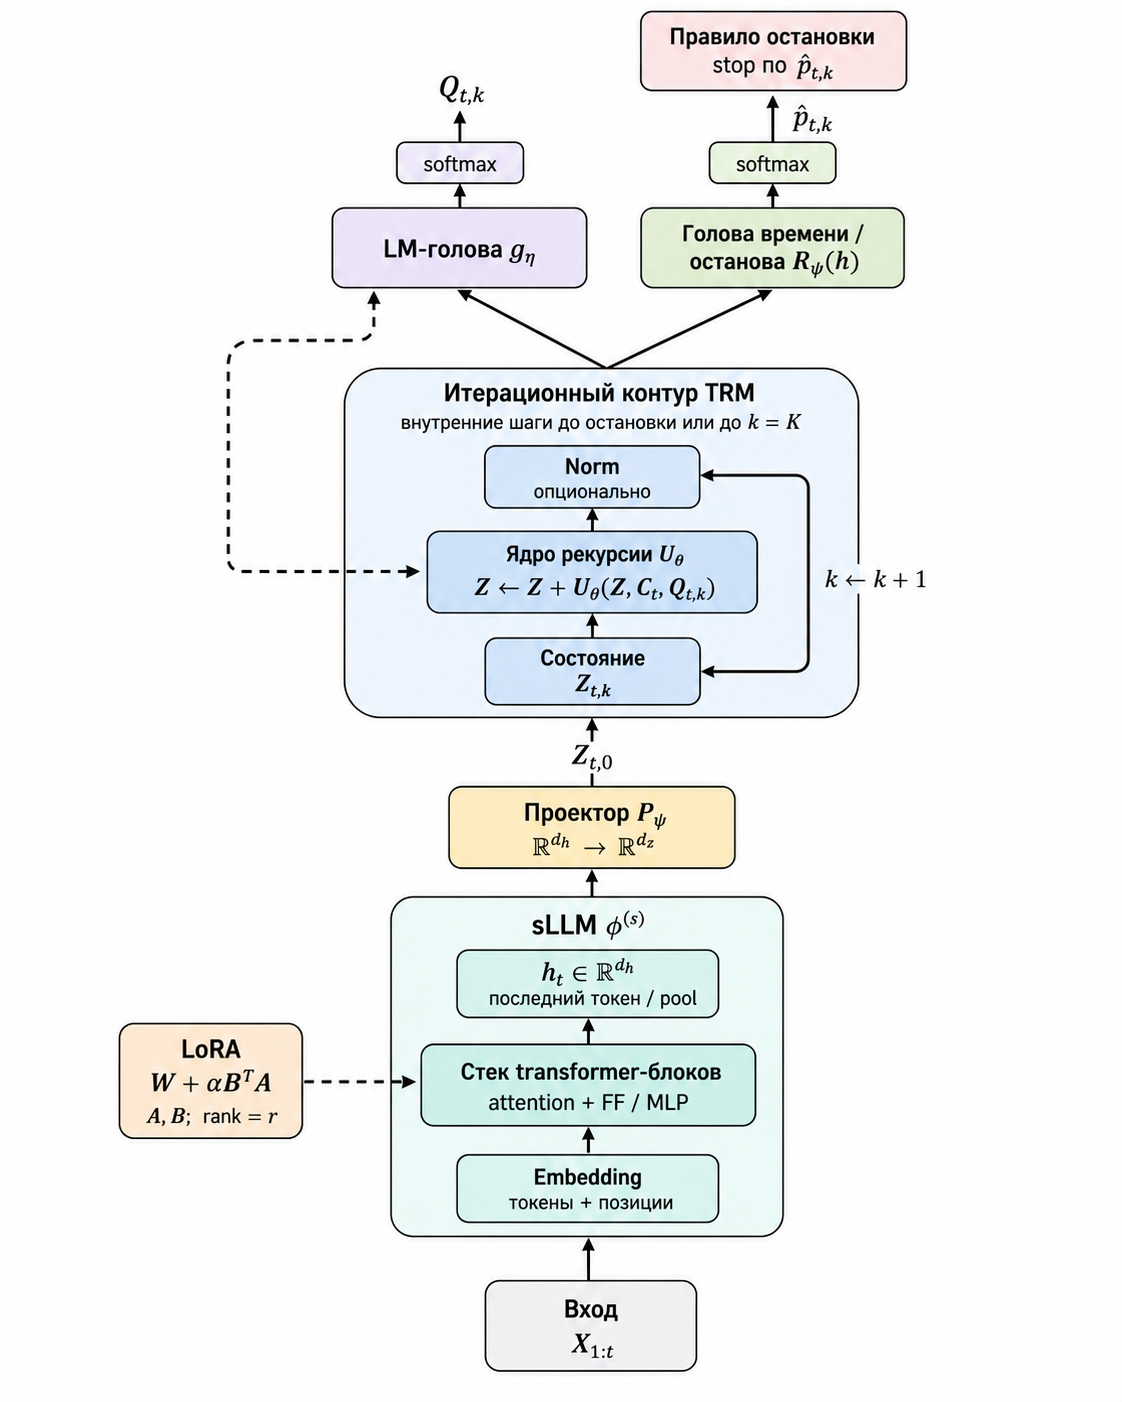
\includegraphics[width=\linewidth]{frozen}
\caption{Структура сети sLLM\,+\,TRM: эмбеддинг и стек трансформерных блоков (опционально с
LoRA~\cite{hu2021}) задают \(h_t\), проектор \(P_\psi\) переводит в \(Z_{t,0}\); далее --- то же
рекурсивное ядро и головы, что на рис.~\ref{fig:arch_trm_oracle}. Обучение по оракульной разметке
описано текстом выше.}
\label{fig:arch_sllm_trm}
\end{figure}

Обобщённый параметр одной сборки композции запишется как наложение ограничений
\[
  \Theta = \bigl(\phi^{\mathrm{(s)}},\psi,\theta,\eta,\omega,\text{ возможно члены LoRA }\bigr)
\]
с разнесением множества обучения по задачам: ядро и головы TRM традиционно включаются в каждый
градиентный шаг, параметры \(\phi^{\mathrm{(s)}}\) и LoRA включаются выборочно.
